\documentclass[11pt,a4paper]{article}

\usepackage[margin=2.2cm]{geometry}
\usepackage[T1]{fontenc}
\usepackage[utf8]{inputenc}
\usepackage{lmodern}
\usepackage{amsmath,amssymb}
\usepackage{enumitem}
\usepackage{array}
\usepackage{booktabs}
\usepackage{multicol}
\usepackage{lastpage}
\usepackage{fancyhdr}
\usepackage{placeins}
\usepackage{setspace}
\usepackage{parskip}
\usepackage{pgfplots}
\pgfplotsset{compat=1.18}
\usepackage{tikz}

\begin{document}
\pagestyle{fancy}
\fancyhf{}  % Clear default headers and footers
\renewcommand{\headrulewidth}{0pt}  % No top horizontal line
\renewcommand{\footrulewidth}{0pt}  % No bottom horizontal line
\fancyfoot[R]{\thepage/\pageref{LastPage}}  % Right footer: X/Y format
\fancypagestyle{plain}{
    \fancyhf{}  % Clear default first-page footer
    \fancyfoot[R]{\thepage/\pageref{LastPage}}  % Apply the same footer
    \renewcommand{\headrulewidth}{0pt}  % Remove top line on first page
    \renewcommand{\footrulewidth}{0pt}  % Ensure no bottom line
}
\title{5731.25 Wireless Communication}
\date{24. March 2025}
\maketitle

\section*{Instructions to Students}

\begin{itemize}
    \item Ensure clarity and precision in your answers.
    \item Attempt all sections. Each of the three sections contributes one-third (1/3) of the total mark.
    \item All answers must be written in \textbf{English}.
    \item Write your answers in the provided answer sheets using a pen.
    \item Each page must contain your name and student number.
    \item Number all submitted pages as \textit{Page X/Y}, where \textit{X} is the page number and \textit{Y} is the total (e.g., \textit{1/9, 2/9, ..., 9/9} for nine pages). 
    \item For the multiple-choice section, indicate your answers using the format: Q1 A, Q2 C, ...
    \item In the appendix of this document, you will find a logarithm tables for reference.
\end{itemize}
\newpage
\section*{Section 1 --- Multiple Choice (20 questions)}

Choose the \textbf{one best answer} for each question.

\vspace{0.3cm}

\begin{multicols}{2}
\begin{enumerate}[leftmargin=*, itemsep=0.4em]

\item Which statement best describes the Fourier transform?
\begin{enumerate}[label=\alph*)]
\item Converts frequency to power
\item Relates time and frequency domains
\item Removes noise
\item Increases gain
\end{enumerate}

\item Thermal noise density at room temperature is approximately:
\begin{enumerate}[label=\alph*)]
\item $-174$ dBm/Hz
\item $-147.6$ dBm/Hz
\item $0$ dBm/Hz
\item $+10$ dBm/Hz
\end{enumerate}

\item Shannon capacity is:
\begin{enumerate}[label=\alph*)]
\item $C = B\log_{10}(1+\mathrm{SNR})$
\item $C = B\log_2(1+\mathrm{SNR})$
\item $C = \mathrm{SNR}\log_2(B)$
\item $C = B/(1+\mathrm{SNR})$
\end{enumerate}

\item Increasing bandwidth (fixed $P_t$) leads to:
\begin{enumerate}[label=\alph*)]
\item lower noise
\item higher noise
\item lower path loss
\item higher antenna gain
\end{enumerate}

\item Which is a multiple access technique?
\begin{enumerate}[label=\alph*)]
\item AWGN
\item Friis equation
\item Rayleigh fading
\item OFDMA
\end{enumerate}

\item Noise figure represents:
\begin{enumerate}[label=\alph*)]
\item antenna gain
\item path loss
\item SNR degradation in receiver
\item bandwidth
\end{enumerate}

\item Which effect bends waves around obstacles?
\begin{enumerate}[label=\alph*)]
\item Reflection
\item Diffraction
\item Absorption
\item Duplexing
\end{enumerate}

\item A wireless link is feasible if:
\begin{enumerate}[label=\alph*)]
\item $P_t > 0$
\item $G_t = G_r$
\item SINR exceeds threshold
\item $f < 1$ GHz
\end{enumerate}

\item Free-space path loss:
\begin{enumerate}[label=\alph*)]
\item decreases with distance
\item decreases with frequency
\item is constant
\item increases with both
\end{enumerate}

\item Short-range low-power wireless technology:
\begin{enumerate}[label=\alph*)]
\item BLE
\item WiFi
\item LTE
\item Satellite
\end{enumerate}

\item Which of the following is a common use of hashing in wireless security?
\begin{enumerate}[label=\alph*)]
\item Message integrity
\item Signal modulation
\item Frequency reuse
\item Beamforming
\end{enumerate}

\item Multipath is caused by:
\begin{enumerate}[label=\alph*)]
\item noise only
\item reflections and delays
\item modulation
\item coding
\end{enumerate}

\item Channel variation speed relates to:
\begin{enumerate}[label=\alph*)]
\item coherence time
\item antenna size
\item bandwidth
\item noise figure
\end{enumerate}

\item Frequency reuse is used to:
\begin{enumerate}[label=\alph*)]
\item remove interference
\item reduce noise
\item avoid modulation
\item increase spectral efficiency
\end{enumerate}

\item Relays \textcolor{red}{!! Anssa eftir}:
\begin{enumerate}[label=\alph*)]
\item always reduce delay
\item improve coverage
\item remove interference
\item only for wired systems
\end{enumerate}

\item Security in wireless involves:
\begin{enumerate}[label=\alph*)]
\item authentication
\item routing
\item shadowing
\item reuse factor
\end{enumerate}

\item Beamforming:
\begin{enumerate}[label=\alph*)]
\item spreads power equally
\item removes antennas
\item steers energy directionally
\item only works at low freq
\end{enumerate}

\item OFDMA enables multiple users to share the channel by:
\begin{enumerate}[label=\alph*)]
\item Allocating different subcarriers and time slots
\item Using only time division
\item Using only frequency division
\item Avoiding scheduling
\end{enumerate}

\item Licensed spectrum example:
\begin{enumerate}[label=\alph*)]
\item NB-IoT
\item LoRaWAN
\item Sigfox
\item Zigbee
\end{enumerate}

\item Which of the following is characteristic of licensed spectrum?
\begin{enumerate}[label=\alph*)]
\item High interference
\item Free access
\item No regulation
\item Exclusive use
\end{enumerate}

\end{enumerate}
\end{multicols}
\newpage

\section*{Section 2 --- Short Questions (6 questions)}

Answer briefly but clearly.

\begin{enumerate}[leftmargin=0.9cm]

\item Write the free-space path loss formula in dB form and explain each term.

\item Explain the difference between licensed and unlicensed spectrum. Give one example of each.

\begin{enumerate}[label=\alph*)]
    \item Explain why interference is more likely in unlicensed spectrum.
    \item Describe one mechanism used to reduce collisions in such systems.
\end{enumerate}

\item What is SINR, and why is it often more useful than SNR in multi-user wireless systems?

\item Explain why increasing bandwidth does not always give a increase in capacity.

\item Briefly explain one important security challenge in wireless or IoT systems, and mention one mechanism used to address it.

\item A base station uses beamforming.

\begin{enumerate}[label=\alph*)]
    \item Explain how beamforming improves signal quality for a user.
    \item Explain one potential limitation of beamforming.
\end{enumerate}
\end{enumerate}

\newpage

\section*{Section 3 --- Long / Applied Questions}

\textbf{Show all calculations and reasoning.}

\subsection*{Question 1 --- Link Budget, Feasibility, and Frequency Change}

A transmitter operates at $f = 800$ MHz with:
\begin{itemize}[leftmargin=1.2cm]
    \item transmit power $P_t = 10$ dBm,
    \item transmit antenna gain $G_t = 0$ dBi,
    \item receive antenna gain $G_r = 0$ dBi,
    \item distance $d = 1.0$ km.
    \item Noise figure $\text{NF} = 10$
\end{itemize}

Assume:
\[
N = -120\ \mathrm{dBm}, \qquad \gamma_{\min} = 3\ \mathrm{dB}
\]

\begin{enumerate}[label=\alph*)]
    \item Compute the free-space path loss at 800 MHz.
    \item Compute the received power $P_r$.
    \item Determine the minimum required received power for feasibility.
    \item Is the link feasible?
    \item The carrier frequency is now changed from 800 MHz to 3 GHz, while all other parameters remain unchanged. Compute the new received power at 3 GHz.
\end{enumerate}
\subsection*{Question 2 --- Indoor Propagation with Obstacles}

An indoor wireless link has:
\begin{itemize}[leftmargin=1.2cm]
    \item distance-based path loss of $75$ dB,
    \item two concrete walls causing $10$ dB loss each,
    \item one wooden door causing $3$ dB loss,
    \item one glass window causing $2$ dB loss.
\end{itemize}

The transmitter uses:
\[
P_t = 10\ \mathrm{dBm}, \qquad G_t = 0\ \mathrm{dBi}, \qquad G_r = 0\ \mathrm{dBi}
\]

\begin{enumerate}[label=\alph*)]
    \item Compute the total path loss.
    \item Compute the received power.
    \item If the receiver sensitivity is $-85$ dBm, does the link work?
    \item Describe how increasing frequency affects signal penetration through obstacles.
\end{enumerate}
\newpage
\subsection*{Question 3 --- Frequency Reuse in Cellular Networks}

Figure~\ref{fig:reuse} shows a cellular network with frequency reuse. Each cell is labeled with a number representing its assigned frequency channel.

\begin{figure}[h!]
\centering
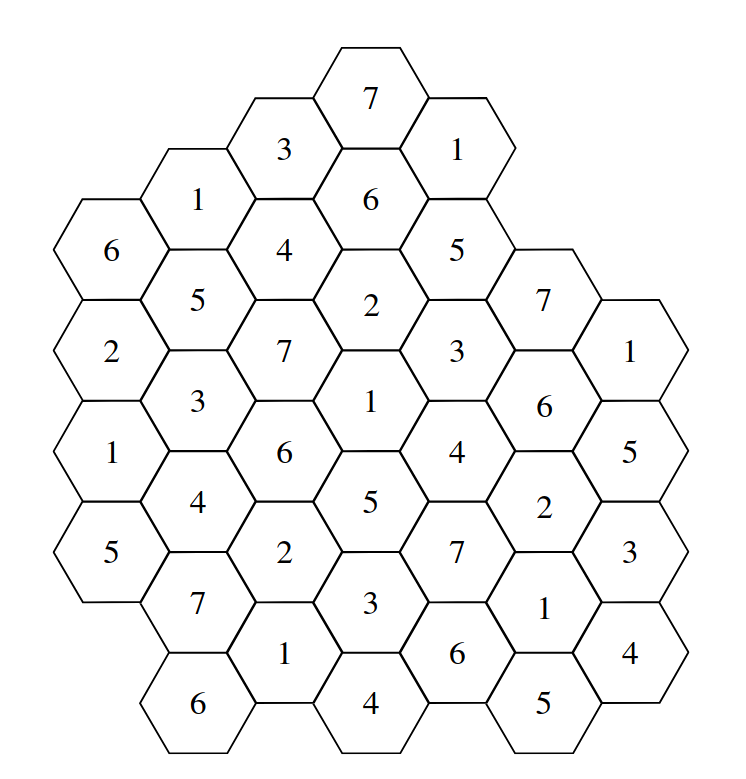
\includegraphics[width=0.6\textwidth]{reuse.png}
\caption{Cellular frequency reuse pattern}
\label{fig:reuse}
\end{figure}


\begin{enumerate}[label=\alph*)]
    \item Determine the frequency reuse factor $N$ for this network.
    \item Determine the values of $(i,j)$ corresponding to this reuse pattern.
    \item Explain how reducing the reuse factor $N$ affects:
    \begin{enumerate}[label=\roman*)]
        \item available bandwidth per cell,
        \item interference between cells.
    \end{enumerate}

\end{enumerate}

\subsection*{Question 4 --- Multi-Hop Routing and Energy}

Consider four nodes: node 1, node 2, node 3, and a gateway $G$.
Only the following links are feasible:

\[
1 \rightarrow 2,\quad 1 \rightarrow 3,\quad 2 \rightarrow 3,\quad 2 \rightarrow G,\quad 3 \rightarrow G
\]

The transmission energy costs are:

\[
E_{12}=2.0,\quad E_{13}=4.8,\quad E_{23}=1.5,\quad E_{2G}=3.1,\quad E_{3G}=2.0
\]

\begin{enumerate}[label=\alph*)]
    \item List all feasible routes from node 1 to the gateway.
    \item Determine the minimum-energy route.
    \item Discuss one advantage and one disadvantage of using multi-hop communication.
\end{enumerate}

\vspace{0.4cm}

\subsection*{Question 5 --- Modulation, Throughput, and Adaptive Coding}

A wireless system operates over a channel with bandwidth $B = 200$ kHz.

Figure~\ref{fig:amc_snr} shows the throughput of several modulation and coding schemes (MCS) as a function of SNR, together with the Shannon capacity bound.

% In preamble:
% \usepackage{pgfplots}
% \pgfplotsset{compat=1.18}

\begin{figure}[h!]
\centering
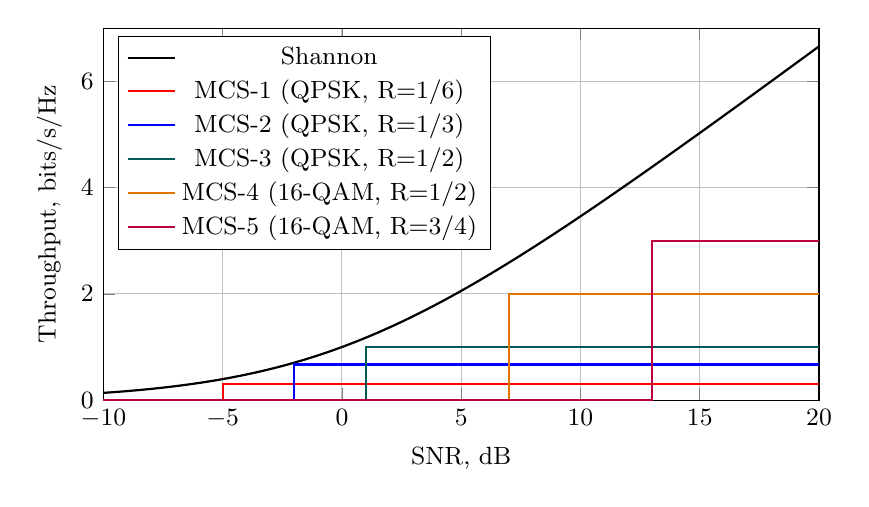
\begin{tikzpicture}
\begin{axis}[
    width=0.88\textwidth,
    height=0.52\textwidth,
    xlabel={SNR, dB},
    ylabel={Throughput, bits/s/Hz},
    xmin=-10, xmax=20,
    ymin=0, ymax=7,
    grid=both,
    major grid style={gray!50},
    minor grid style={gray!20},
    legend style={
        at={(0.02,0.98)},
        anchor=north west,
        fill=white,
        draw=black,
        font=\small
    },
    tick label style={font=\small},
    label style={font=\small},
    every axis plot/.append style={thick}
]

% Shannon
\addplot[domain=-10:20,samples=300,black]
    {ln(1 + 10^(x/10))/ln(2)};
\addlegendentry{Shannon}

% Simple step-like MCS curves
\addplot[red, const plot]
coordinates {
(-10,0) (-5,0) (-5,0.30) (20,0.30)
};
\addlegendentry{MCS-1 (QPSK, R=1/6)}

\addplot[blue, const plot]
coordinates {
(-10,0) (-2,0) (-2,0.67) (20,0.67)
};
\addlegendentry{MCS-2 (QPSK, R=1/3)}

\addplot[teal!70!black, const plot]
coordinates {
(-10,0) (1,0) (1,1.00) (20,1.00)
};
\addlegendentry{MCS-3 (QPSK, R=1/2)}

\addplot[orange!90!black, const plot]
coordinates {
(-10,0) (7,0) (7,2.00) (20,2.00)
};
\addlegendentry{MCS-4 (16-QAM, R=1/2)}

\addplot[purple, const plot]
coordinates {
(-10,0) (13,0) (13,3.00) (20,3.00)
};
\addlegendentry{MCS-5 (16-QAM, R=3/4)}

\end{axis}
\end{tikzpicture}
\caption{Modulation and coding throughput versus SNR.}
\label{fig:amc_snr}
\end{figure}
\FloatBarrier

\begin{enumerate}[label=\alph*)]

\item Assume $\mathrm{SNR} = 10$ dB. Compute the theoretical maximum achievable data rate.

\item Using Figure~\ref{fig:amc_snr}, determine:
\begin{enumerate}[label=\roman*)]
    \item the highest usable MCS at $\mathrm{SNR} = 10$ dB,
    \item its throughput with the given bandwidth.
\end{enumerate}

\item The system currently operates at $\mathrm{SNR} = 12$ dB, with a transmission power of 100 W.

How much can the transmitted signal power be reduced before the selected MCS changes and throughput decreases?

\textit{Assume noise power remains constant.}

\end{enumerate}

\section*{Question 6 --- Base Station Placement and Coverage Analysis}

A wireless operator wants to provide coverage to the two towns shown on the last page, as well as as much of the surrounding terrain as possible.

You must consider both coverage and deployment cost (tower height).

\begin{enumerate}[label=\alph*)]

\item Propose a single-site solution and justify your choice.

\item Propose a multi-site solution (for example, a base station and a relay) and explain how coverage improves.

\item Compare the two solutions in terms of:
coverage, tower height, cost, and reliability.

\item Assume many users are active in one of the towns. Which solution provides better performance? Justify your answer considering medium access and interference.

\item Identify the main propagation effects influencing your design.

\end{enumerate}
\vspace{0.6cm}
\hrule
\vspace{0.3cm}

\textbf{End of exam}


\newpage
\section{Supplemental material}
\subsection{Logarithm Properties}
\begin{itemize}
    \item \textbf{Product Rule:} 
    \[
    \log_b (xy) = \log_b (x) + \log_b (y)
    \]
    \item \textbf{Quotient Rule:} 
    \[
    \log_b \left( \frac{x}{y} \right) = \log_b (x) - \log_b (y)
    \]
    \item \textbf{Power Rule:} 
    \[
    \log_b (x^n) = n \log_b (x)
    \]
    \item \textbf{Base Change Formula:} 
    \[
    \log_b (x) = \frac{\log_c (x)}{\log_c (b)}
    \]
    \item \textbf{Log of Reciprocal:} 
    \[
    \log_b \left( \frac{1}{x} \right) = -\log_b (x)
    \]
    \item \textbf{Logarithm to Exponential Conversion:}
    \[
    x \cdot \log_b(y) = z \quad \Rightarrow \quad y = b^{\frac{z}{x}}
    \]
\end{itemize}
\subsection{Commonly Used Constants and Units}

\begin{itemize}
    \item \textbf{Speed of Light:} 
    \[
    c \approx 3.0 \times 10^8 \text{ m/s}
    \]
    \item \textbf{Boltzmann's Constant:} 
    \[
    k_B = 1.38 \times 10^{-23} \text{ J/K}
    \]
        \item \textbf{Thermal Noise Power Density:}  
    \[
    P_n (1 \text{ Hz}) = -174 \text{ dBm/Hz}
    \]
    
\end{itemize}

\subsection{Conversion Examples}
\begin{itemize}
    \item \(\log_{2} (16) = 4\), since \(2^4 = 16\).
    \item \(\log_{10}(12) = \log_{10}(6)+\log_{10}(2)\)
    \item Converting \( 20 \) dB to a linear factor: \(10^{\frac{20}{10}} = 10^{2} = 100\)
    \item \(10^{1.5} = 10^1 \cdot 10^{0.5} \approx 10 \cdot 3.16 = 31.6\)

\end{itemize}

\begin{table}[h]
    \centering
    \renewcommand{\arraystretch}{1.2}
    \begin{tabular}{|l|r|r|r|r|}
        \hline
        \textbf{Value} & \(\log_{10}(\text{Value})\) & \(\log_{2}(\text{Value})\) & Scientific Notation & SI - Prefix \\
        \hline
        \(10^{-9}\)   & -9.000  & -29.897 & \(1.0 \times 10^{-9}\) & Nano \\
        \(10^{-8}\)   & -8.000  & -26.575 & \(1.0 \times 10^{-8}\) & \\
        \(10^{-7}\)   & -7.000  & -23.253 & \(1.0 \times 10^{-7}\) & \\
        \(10^{-6}\)   & -6.000  & -19.931 & \(1.0 \times 10^{-6}\) & Micro \\
        \(10^{-5}\)   & -5.000  & -16.609 & \(1.0 \times 10^{-5}\) & \\
        \(10^{-4}\)   & -4.000  & -13.287 & \(1.0 \times 10^{-4}\) & \\
        \(10^{-3}\)   & -3.000  & -9.966  & \(1.0 \times 10^{-3}\) & Milli \\
        \(0.01\)   & -2.000  & -6.644  & \(1.0 \times 10^{-2}\) & \\
        \(0.1\)   & -1.000  & -3.322  & \(1.0 \times 10^{-1}\) & \\
        \hline
        1             & 0.000   & 0.000   & \(1.0 \times 10^{0}\) & - \\
        2             & 0.301   & 1.000   & \(2.0 \times 10^{0}\) & \\
        3             & 0.477   & 1.585   & \(3.0 \times 10^{0}\) & \\
        4             & 0.602   & 2.000   & \(4.0 \times 10^{0}\) & \\
        5             & 0.699   & 2.322   & \(5.0 \times 10^{0}\) & \\
        6             & 0.778   & 2.585   & \(6.0 \times 10^{0}\) & \\
        7             & 0.845   & 2.807   & \(7.0 \times 10^{0}\) & \\
        8             & 0.903   & 3.000   & \(8.0 \times 10^{0}\) & \\
        9             & 0.954   & 3.170   & \(9.0 \times 10^{0}\) & \\
        10            & 1.000   & 3.322   & \(1.0 \times 10^{1}\) & \\
        \hline
        \(100\)      & 2.000   & 6.644   & \(1.0 \times 10^{2}\) & \\
        \(1000\)      & 3.000   & 9.966   & \(1.0 \times 10^{3}\) & Kilo \\
        \(10^4\)      & 4.000   & 13.287  & \(1.0 \times 10^{4}\) & \\
        \(10^5\)      & 5.000   & 16.609  & \(1.0 \times 10^{5}\) & \\
        \(10^6\)      & 6.000   & 19.931  & \(1.0 \times 10^{6}\) & Mega \\
        \(10^7\)      & 7.000   & 23.253  & \(1.0 \times 10^{7}\) & \\
        \(10^8\)      & 8.000   & 26.575  & \(1.0 \times 10^{8}\) & \\
        \(10^9\)      & 9.000   & 29.897  & \(1.0 \times 10^{9}\) & Giga \\
        \hline
    \end{tabular}
\end{table}
\newpage
\.\\
\newpage

\begin{center}
\textbf{\Large Answer Page – Coverage Design}
\end{center}

\vspace{0.5cm}

\noindent
\textbf{Name:} \rule{6cm}{0.4pt}
\hfill
\textbf{Page} [\ \ \ ] \textbf{of} [\ \ \ ]

\vspace{0.8cm}

\textbf{Single-site solution (mark base station and sketch coverage):}\\
Red crosses indicate town location. 
\vspace{0.3cm}

\begin{center}
\begin{tikzpicture}[scale=0.7]

% Axes
\draw[->] (0,-0.5) -- (21,-0.5) node[right] {Distance};
\draw[->] (0,-0.5) -- (0,8) node[above] {Height};

% Terrain
\draw[thick] 
(0,0.5) -- (1,0.3) -- (2,0.4) -- (3,0.6)
-- (4,1.5) -- (5,3.0) -- (6,4.0) -- (7,4.3)
-- (8,4.2) -- (8.5,3.8) -- (9,2.0)
-- (10,1.8) -- (11,1.7) -- (12,1.8)
-- (13,2.5) -- (14,5.7) -- (15,5.7)
-- (16,4.8) -- (17,4.6) -- (18,5.2)
-- (19,6.0) -- (20,7.0);

% Town A
\draw[red, thick] (2.5,0.5) -- (3.2,1.0);
\draw[red, thick] (3.2,0.5) -- (2.5,1.0);

% Town B
\draw[red, thick] (9.5,1.5) -- (10.2,2.0);
\draw[red, thick] (10.2,1.5) -- (9.5,2.0);

\end{tikzpicture}
\end{center}

\vspace{0.8cm}

\textbf{Multi-site solution with relay (mark base stations and sketch coverage):}

\vspace{0.3cm}

\begin{center}
\begin{tikzpicture}[scale=0.7]

% Axes
\draw[->] (0,-0.5) -- (21,-0.5) node[right] {Distance};
\draw[->] (0,-0.5) -- (0,8) node[above] {Height};

% Terrain
\draw[thick] 
(0,0.5) -- (1,0.3) -- (2,0.4) -- (3,0.6)
-- (4,1.5) -- (5,3.0) -- (6,4.0) -- (7,4.3)
-- (8,4.2) -- (8.5,3.8) -- (9,2.0)
-- (10,1.8) -- (11,1.7) -- (12,1.8)
-- (13,2.5) -- (14,5.7) -- (15,5.7)
-- (16,4.8) -- (17,4.6) -- (18,5.2)
-- (19,6.0) -- (20,7.0);

% Town A
\draw[red, thick] (2.5,0.5) -- (3.2,1.0);
\draw[red, thick] (3.2,0.5) -- (2.5,1.0);

% Town B
\draw[red, thick] (9.5,1.5) -- (10.2,2.0);
\draw[red, thick] (10.2,1.5) -- (9.5,2.0);

\end{tikzpicture}
\end{center}

\vfill

\hrule
\vspace{0.3cm}
\textit{Clearly indicate base station locations and draw approximate coverage areas.}

\clearpage
\label{LastPage}

%\section*{Suggested Solutions}

\subsection*{Section 1 --- Multiple Choice}

\begin{center}
\begin{tabular}{cccccccccc}
1:b & 2:a & 3:b & 4:b & 5:b & 6:b & 7:b & 8:c & 9:c & 10:a \\
11:a & 12:b & 13:a & 14:b & 15:b & 16:a & 17:b & 18:a & 19:a & 20:a
\end{tabular}
\end{center}

\vspace{0.5cm}

\subsection*{Section 2 --- Short Answers}

\begin{enumerate}[leftmargin=0.9cm]

\item 
\[
L_{\mathrm{FSPL}} = 32.44 + 20\log_{10}(f_{\mathrm{MHz}}) + 20\log_{10}(d_{\mathrm{km}})
\]
Frequency $\uparrow$ $\Rightarrow$ loss $\uparrow$, distance $\uparrow$ $\Rightarrow$ loss $\uparrow$.

\item 
Licensed: exclusive use (e.g., NB-IoT).  
Unlicensed: shared (e.g., LoRa/WiFi).  

a) More users $\Rightarrow$ more interference.  
b) Example: CSMA / listen-before-talk.

\item 
\[
\mathrm{SINR} = \frac{S}{N+I}
\]
Includes interference, more realistic than SNR.

\item 
Increasing bandwidth increases noise power $\Rightarrow$ SNR decreases $\Rightarrow$ diminishing capacity gain.

\item 
Example: eavesdropping or spoofing.  
Solution: encryption or authentication.

\item 
Beamforming focuses energy $\Rightarrow$ higher SNR, less interference.  
Limitation: requires channel knowledge, sensitive to mobility.

\end{enumerate}

\vspace{0.5cm}

\subsection*{Section 3 --- Long Questions}

\subsubsection*{Question 1}

a)
\[
L = 32.44 + 20\log_{10}(800) \approx 90.5\ \mathrm{dB}
\]

b)
\[
P_r = 15 + 2 + 2 - 90.5 = -71.5\ \mathrm{dBm}
\]

c)
\[
P_{\min} = -120 + 3 = -117\ \mathrm{dBm}
\]

d) Feasible ($-71.5 > -117$)

e)
\[
L_{3\,\mathrm{GHz}} \approx 102\ \mathrm{dB}, \quad P_r \approx -83\ \mathrm{dBm}
\]

f) Higher frequency $\Rightarrow$ higher path loss.

\vspace{0.3cm}

\subsubsection*{Question 2}

a)
\[
L_{\text{total}} = 75 + 20 + 3 + 2 = 100\ \mathrm{dB}
\]

b)
\[
P_r = 10 - 100 = -90\ \mathrm{dBm}
\]

c) Not feasible ($-90 < -85$)

d) Loss depends on material properties and frequency.

\vspace{0.3cm}

\subsubsection*{Question 3}

a) $N = 7$

b) $(i,j) = (2,1)$

c)
\begin{itemize}
\item Bandwidth per cell increases as $N$ decreases
\item Interference increases as $N$ decreases
\end{itemize}

\vspace{0.3cm}

\subsubsection*{Question 4}

a)
\[
N = 10^{-12}\ \mathrm{mW}, \quad I \approx 1.58\times 10^{-11}\ \mathrm{mW}
\]

b)
\[
N+I \approx 1.68\times10^{-11} \Rightarrow -107.7\ \mathrm{dBm}
\]

c)
\[
\mathrm{SINR} = -95 - (-107.7) = 12.7\ \mathrm{dB}
\]

d) Feasible ($12.7 > 5$)

e) Many users $\Rightarrow$ interference dominates.

\vspace{0.3cm}

\subsubsection*{Question 5}

a)
\begin{itemize}
\item $1 \rightarrow 2 \rightarrow G$
\item $1 \rightarrow 2 \rightarrow 3 \rightarrow G$
\item $1 \rightarrow 3 \rightarrow G$
\end{itemize}

b)
\[
5.1,\quad 5.5,\quad 6.8
\]

c) Minimum: $1 \rightarrow 2 \rightarrow G$

d) Shorter hops reduce path loss.

e) Advantage: lower power. Disadvantage: delay/complexity.

\vspace{0.3cm}

\subsubsection*{Question 6}

a)
\[
C = 200\,\mathrm{kHz} \cdot \log_2(11) \approx 200 \cdot 3.46 = 692\ \mathrm{kbps}
\]

b)
MCS $\approx$ QPSK, $R=1/2$, throughput $\approx 1$ bit/s/Hz

c)

Threshold $\approx 8$ dB

\[
\Delta = 12 - 8 = 4\ \mathrm{dB}
\]

\[
\text{Power factor} = 10^{4/10} \approx 2.51
\]

\[
P_{\min} \approx \frac{100}{2.51} \approx 40\ \mathrm{W}
\]

Reduction $\approx 60\ \mathrm{W}$

\vspace{0.3cm}

\subsubsection*{Question 7}

a) Place BS at elevated position for LOS.

b) Two-site/relay improves coverage in shadowed regions.

c)
\begin{itemize}
\item Two-site: better coverage, lower tower
\item Single-site: cheaper but more shadowing
\end{itemize}

d) Two-site better: load split, less interference/medium access contention.

e) Path loss, shadowing, diffraction.

\end{document}